\documentclass[
% -- opções da classe memoir --
12pt,				% tamanho da fonte
% openright,			% capítulos começam em pág ímpar (insere página vazia caso preciso)
oneside,			% para impressão em recto e verso. Oposto a oneside
a4paper,			% tamanho do papel.
% -- opções da classe abntex2 --
section=TITLE,
% subsection=TITLE,
% section=TITLE,		% títulos de seções convertidos em letras maiúsculas
% section=TITLE,
%subsection=TITLE,	% títulos de subseções convertidos em letras maiúsculas
%subsubsection=TITLE,% títulos de subsubseções convertidos em letras maiúsculas
% -- opções do pacote babel --
% sumario=tradicional
brazil,				% o último idioma é o principal do documento
]{abntex2}

% ---
% PACOTES
% ---

% ---
% Pacotes fundamentais
% ---
% Fonte ARIAL
\usepackage{helvet}
\renewcommand{\familydefault}{\sfdefault}
%------
% \usepackage{lmodern}			% Usa a fonte Latin Modern
\usepackage[T1]{fontenc}		% Selecao de codigos de fonte.
\usepackage[utf8]{inputenc}		% Codificacao do documento (conversão automática dos acentos)
\usepackage{indentfirst}		% Indenta o primeiro parágrafo de cada seção.
\usepackage{color}				% Controle das cores
\usepackage{graphicx}			% Inclusão de gráficos
\usepackage{microtype} 			% para melhorias de justificação
% ---

%Para links
\usepackage{hyperref}
% ---
% Pacotes adicionais, usados apenas no âmbito do Modelo Canônico do abnteX2
% ---
\usepackage{lipsum}				% para geração de dummy text
% ---

% ---
% Pacotes de citações
% ---
\usepackage[brazilian,hyperpageref]{backref}	 % Paginas com as citações na bibl
\usepackage[alf]{abntex2cite}	% Citações padrão ABNT

% ---
% CONFIGURAÇÕES DE PACOTES
% ---

%% Estilizando section
\usepackage{titlesec}
\titleformat{\section}    {\normalfont\fontfamily{phv}\fontsize{12}{17}\bfseries}{\thesection}{1em}{}
\renewcommand{\ABNTEXsectionfontsize}{\normalsize}
\titleformat{\subsection}    {\normalfont\fontfamily{phv}\fontsize{12}{17}\bfseries}{\thesubsection}{1em}{}
\renewcommand{\ABNTEXsectionfontsize}{\normalsize}
%----

% ---
% Configurações do pacote backref
% Usado sem a opção hyperpageref de backref
\renewcommand{\backrefpagesname}{Citado na(s) página(s):~}
% Texto padrão antes do número das páginas
\renewcommand{\backref}{}
% Define os textos da citação
\renewcommand*{\backrefalt}[4]{
  \ifcase #1 %
    % Nenhuma citação no texto.%
    \or
    % Citado na página #2.%
  \else
    % Citado #1 vezes nas páginas #2.%
  \fi}%
  % ---
  % Novo list of (listings) para QUADROS

  \newcommand{\quadroname}{Quadro}
  \newcommand{\listofquadrosname}{Lista de quadros}

  \newfloat[section]{quadro}{loq}{\quadroname}
  \newlistof{listofquadros}{loq}{\listofquadrosname}
  \newlistentry{quadro}{loq}{0}

  % configurações para atender às regras da ABNT
  \setfloatadjustment{quadro}{\centering}
  \counterwithout{quadro}{section}
  \renewcommand{\cftquadroname}{\quadroname\space}
  \renewcommand*{\cftquadroaftersnum}{\hfill--\hfill}

  % Configuração de posicionamento padrão:
  \setfloatlocations{quadro}{hbtp}

  % opção para Artigo
  \counterwithout{section}{section}
  \counterwithout{figure}{section}
  \counterwithout{table}{section}
  \renewcommand{\footnotesize}{\small}



  % ---
  % Informações de dados para CAPA e FOLHA DE ROSTO
  % ---
  \titulo{Projeto Integrado Multidisciplinar V}
  \autor{ UNIP EaD\\
    Andreia Domingues da Silva RA: 2023727\\
  Pedro Expedito De Oliveira RA: 2028118}
  \local{Santa Fé-PR}
  \data{2021}
  \instituicao{%
    Universidade Paulista -- Unip
    \par
    Faculdade de Analise e Desenvolvimento Sistemas
    \par
  Projeto Integrado Multidisciplinar}
  \tipotrabalho{Tese (Doutorado)}
  % O preambulo deve conter o tipo do trabalho, o objetivo,
  % o nome da instituição e a área de concentração
  \preambulo{Projeto Integrado Multidisciplinar para obtenção do título de tecnólogo
    em Análise e Desenvolvimento de Sistemas apresentado à Universidade Paulista – UNIP EaD.\\
  Orientador(a): .}
  % ---

  % ---
  % Configurações de aparência do PDF final

  % alterando o aspecto da cor azul
  \definecolor{blue}{RGB}{41,5,195}

  % informações do PDF
  \makeatletter
  \hypersetup{
    %pagebackref=true,
    pdftitle={\@title},
    pdfauthor={\@author},
    pdfsubject={\imprimirpreambulo},
    pdfcreator={LaTeX with abnTeX2},
    pdfkeywords={abnt}{latex}{abntex}{abntex2}{PIM},
    colorlinks=true,       		% false: boxed links; true: colored links
    linkcolor=blue,          	% color of internal links
    citecolor=blue,        		% color of links to bibliography
    filecolor=magenta,      		% color of file links
    urlcolor=blue,
    bookmarksdepth=4
  }
  \makeatother
  % ---

  % ---
  % Espaçamentos entre linhas e parágrafos
  % ---

  % O tamanho do parágrafo é dado por:
  \setlength{\parindent}{1.3cm}

  % Controle do espaçamento entre um parágrafo e outro:
  \setlength{\parskip}{0.2cm}  % tente também \onelineskip

  % ---
  % compila o indice
  % ---
  % \makeindex
  % ---

  % ----
  % Início do documento
  % ----
  % \setlength\afterchapskip{\lineskip}
  %quebra de pagina
  \let\oldsection\section
  \renewcommand\section{\clearpage\oldsection}
  \begin{document}


  % Seleciona o idioma do documento (conforme pacotes do babel)
  \selectlanguage{brazil}

  % Retira espaço extra obsoleto entre as frases.
  \frenchspacing

  % ----------------------------------------------------------
  % ELEMENTOS PRÉ-TEXTUAIS
  % ----------------------------------------------------------
  % \pretextual

  % ---
  % Capa
  % ---
  \imprimircapa
  % ---

  % ---
  % Folha de rosto
  % ---
  \imprimirfolhaderosto
  % ---

  % ---
  % NOTA DA ABNT NBR 15287:2011, p. 4:
  %  ``Se exigido pela entidade, apresentar os dados curriculares do autor em
  %     folha ou página distinta após a folha de rosto.''
  % ---

  % ---
  % inserir lista de ilustrações
  % ---
  % \pdfbookmark[0]{\listfigurename}{lof}
  % \listoffigures*
  % \cleardoublepage
  % ---

  % ---
  % inserir lista de tabelas
  % ---
  % \pdfbookmark[0]{\listtablename}{lot}
  % \listoftables*
  % \cleardoublepage
  % % ---

  % ---
  % inserir lista de abreviaturas e siglas
  % ---
  % \begin{siglas} \item[ABNT] Associação Brasileira de Normas Técnicas
  % \item[abnTeX] ABsurdas Normas para TeX
  % \end{siglas}
  % ---

  % ---
  % inserir lista de símbolos
  % ---
  % \begin{simbolos}
  %   \item[$ \Gamma $] Letra grega Gama
  %   \item[$ \Lambda $] Lambda
  %   \item[$ \zeta $] Letra grega minúscula zeta
  %   \item[$ \in $] Pertence
  % \end{simbolos}
  % ---


  \begin{resumo}

    Este projeto visa resolver o problema do Colégio Vencer Sempre que
    disponibiliza recursos de informática e vídeo  (tais como datashow, TV com VCR,
    TV com DVD, Projetor de Slides, Sistemas de Áudio-Microfone, Caixa Amplificada,
    Notebooks, Kits Multimídia etc.) Utilizando-se das disciplinas economia e
    mercado, Engenharia de Software II, Projeto de Interface com o Usuário e
    Programação Orientada a Objetos I. Desenvolvendo um sistema capaz de facilitar
    e automatizar o empréstimo de equipamentos  e recursos para os professores dos
    do ensino fundamental, médio e superior, cumprindo todos os requisitos de
    software e com o padrão de qualidade da norma ISO 9126 que tem como objetivo a
    qualidade do produto de software. Seguindo as regras de negócio do colégio,
    estabelecendo requisitos funcionais e não funcionais, criando roteiros de
    testes e com interfaces de usuário de alta fidelidade desenvolvidas com a
    ferramenta HTML5 muito utilizada na web. Em economia foi verificado os agentes
    econômicos viabilidade econômica e custos de produção do software.

    \textbf{Palavras-chave}: Sistema. Automatização. Empréstimos.
  \end{resumo}


  % resumo em inglês
  \begin{resumo}[Abstract]
    \begin{otherlanguage*}{english}
      This project aims to solve the problem of Colégio Vencer Whenever it
      provides computer and video resources (such as datashow, TV with VCR, TV
      with DVD, Slide Projector, Audio-Microphone Systems, Amplified Box,
      Notebooks, Multimedia Kits, etc.) Using the economics and market
      disciplines, Software Engineering II, User Interface Design and Object
      Oriented Programming I. Developing a system capable of facilitating and
      automating the loan of equipment and resources for elementary, middle and
      high school teachers superior, fulfilling all the requirements of the
      software and with the quality standard of the norm ISO 9126 that has as
      objective the quality of the software product. Following the school's
      business rules, setting requirements and not doing it, creating test scripts
      and with high-fidelity user interfaces developed with an HTML5 tool widely
      used on the web. In economics the economic agents were verified economic
      viability and costs of production of the software.
      \\
      \vspace{\onelineskip}
      \noindent
      \textbf{Keywords}: System. Automation. Loans.
    \end{otherlanguage*}
  \end{resumo}


  % ---
  % inserir o sumario
  % ---
  \pdfbookmark[0]{\contentsname}{toc}
  \tableofcontents*
  \cleardoublepage
  % ---
  % ----------------------------------------------------------
  % ELEMENTOS TEXTUAIS
  % ----------------------------------------------------------
  \textual

  %Remover sumario do cabeçalho

  \pagestyle{simple}
  \aliaspagestyle{section}{simple}

  % altera o espaçamento depois do número de cada secao, subsecao, etc.
  %altera tamanho de fonte, negrito, itálico, etc.

  % -------

  % ----------------------------------------------------------
  % Introdução
  % ----------------------------------------------------------
  \section{INTRODUÇÃO}

  O Colégio Vencer sempre com o aumento da disponibilização de recursos de
  informática e vídeo precisam de um sistema capaz de fazer a gerência dos
  professores que emprestarem o equipamento. O Sistema vai possuir informações
  como data de empréstimo, data de devolução, status do empréstimo e qual usuário
  emprestou e para maior qualidade no produto final vai ser seguido o padrão da
  ISO ISO 9126 que descreve o modelo de qualidade de software. Com isso, gerando
  um software de maior qualidade e eficiência para que os usuários  possam
  utilizar os equipamentos nas  aulas e em outras atividades. A ferramenta para
  desenvolvimento da interface optou-se pelo HTML5, muito utilizado na web e suas
  maiores vantagens são compatibilidade com mobile, acessibilidade, maior alcance
  e uma incrível facilidade na edição.

  % ----------------------------------------------------------
  % Capitulo de textual
  % ----------------------------------------------------------

  \section{INTERFACE DO USUÁRIO}

  A interface do usuário possuirá para registrar o empréstimo de equipamento para
  os professores, cancelar, editar data de entrega, mudar status. Com o principal
  objetivo de ser fácil de aprender e com boa usabilidade.  Para Nielsen (1993) a
  usabilidade está inserida na aceitação do sistema pelo usuário, que é
  basicamente o sistema ser suficientemente bom para satisfazer todas as
  necessidades e requerimentos de seus usuários.  A ferramenta utilizada vai ser
  HTML que segundo \cite[p.11]{prescott2015html} Html é uma linguagem de marcação utilizada na
  web de fácil aprendizado sendo o bloco básico da construção de uma página.

  % ----------------------------------------------------------
  % Capitulo com exemplos de comandos inseridos de arquivo externo
  % ----------------------------------------------------------

  \include{abntex2-modelo-include-comandos}

  % ---
  % Finaliza a parte no bookmark do PDF
  % para que se inicie o bookmark na raiz
  % e adiciona espaço de parte no Sumário
  % ---
  \phantompart


  \subsection{agendar empréstimo}

  Para o usuário agendar um empréstimo de equipamento o software vai prover uma
  interface gráfica onde haverá os campos de usuário, data e selecionar
  equipamento para empréstimo como demonstra a figura abaixo.

  \begin{figure}[htb]
    \caption{\label{}Registrar empréstimo}
    \begin{center}
      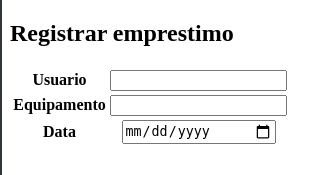
\includegraphics[scale=1.10]{./img/agendar.png}
    \end{center}
    \legend{Fonte: Os Autores (interface de usuário, 2021).}
  \end{figure}

  Os campos são:\\

  \begin{itemize}
    \item \textbf{Usuário:} é a  informação do professor que fez o empréstimo do
      equipamento.

    \item \textbf{Equipamento:} é o equipamento que vai ser emprestado pelo
      usuário.

      \item \textbf{Data:} data que foi feito o empréstimo, já data de entrega
      poderá ser escolhida pelos colégios de acordo com suas políticas como prazo
      máximo de entrega até 15 dias após o empréstimo, sendo escolhida a
      instituição a data de entrega.
  \end{itemize}
  \subsection{Cancelar empréstimo}

  Em caso de erro do administrador ao cadastrar um usuário erroneamente o sistema
  proverá a possibilidade  de cancelamento para que nenhuma das partes seja
  lesada, como mostra na figura abaixo:

  \begin{figure}[htb]
    \caption{\label{}Cancelar empréstimo}
    \begin{center}
      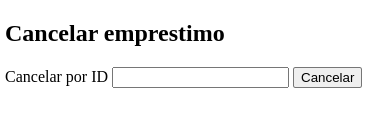
\includegraphics[scale=1.00]{./img/cancelar-imprestimo.png}
    \end{center}
    \legend{Fonte: Os Autores (interface de usuário, 2021).}
  \end{figure}

  Desta forma o administrador insere a identificação do empréstimo e o cancela.

  \subsection{Editar empréstimo}

  Caso alguma mudança seja feita no empréstimo de equipamento de um usuário, como
  data de entrega de entrega ser antecipada ou prorrogado, o administrador poderá
  alterá-lo.

  \begin{figure}[htb]
    \caption{\label{fig_circulo}Editar empréstimo}
    \begin{center}
      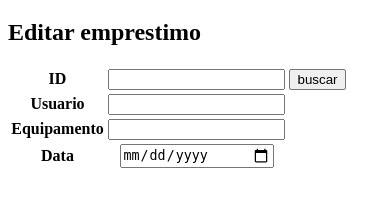
\includegraphics[scale=1]{./img/editar.png}
    \end{center}
    \legend{Fonte: Os Autores (interface de usuário, 2021).}
  \end{figure}

  \textbf{ID:} Identificação do empréstimo gerado automaticamente pelo sistema.

  \textbf{Usuário, Equipamento, Data}  são Preenchidos automaticamente após o
  administrador inserir o ID e clicar no botão `buscar'

  \subsection{Status do Empréstimo}

  Para consultas o sistema fornecerá uma tela para que o administrador do sistema
  tenha visão rápida de como está a situação dos empréstimos, mostrando uma lista
  de todos os empréstimos feitos e de quais equipamentos estão disponíveis para
  emprestar, e os que estão prestes a ser entregues.

  \section{METODOLOGIA APLICADA AO PROJETO}

  A metodologia escolhida para o projeto foi a “ÁGIL” por ser um projeto de
  pequeno porte e possuir muitas vantagens como escopo iterativo, time box e ser
  flexível a mudanças além de ser muito personalizável.  A metodologia ágil
  escolhida vai ser Scrum é a metodologia ágil mais conhecida por ser um
  framework no qual a execução do projeto é feita em sprints ou seja pequenos
  ciclos de trabalho que geram entregas.

  \cite[p.8]{sabbagh2014scrum}Defende que Scrum:

  \begin{citacao}

    Scrum superou métodos tradicionais e tornou-se a forma mais bem-sucedida de
    gestão de projetos de desenvolvimento de software. Este livro mostra como os
    papéis, artefatos, eventos e regras do Scrum, aliados a diversas práticas já
    consagradas, podem ajudar organizações a entregar valor frequentemente para
    seus clientes com menos riscos, com menor desperdício e com maior qualidade,
    visibilidade e produtividade.\cite[p,8]{sabbagh2014scrum}

  \end{citacao}

  Conclui se que Scrum vai cumprir todos os requisitos de gerência para o
  desenvolvimento do software em questão.

  \subsection{Requisitos do sistema}

  Definir os requisitos de um sistema é uma tarefa essencial que pode ser difícil
  e complexa principalmente se o sistema for novo sendo muito difícil definir com
  clareza oque o sistema deve fazer.  Para\cite{sommerville2008engenharia} esses dois níveis
  de requisitos e a especificação de projeto de software podem ser definidos do
  seguinte modo:

  \begin{citacao}
    Requisitos de usuário são declarações em linguagem natural e diagramas
    contendo as funcionalidades e as restrições sob as quais o sistema deve
    operar.
    Esse documento é escrito para gerentes do cliente e dos fornecedores
    que não tenham conhecimento técnico detalhado do sistema.  Requisitos de
    sistema detalham funcionalidades e restrições. Esse documento pode inclusive
    servir como um contrato entre as partes envolvidas no projeto.
    Ele é escrito para os profissionais técnicos de nível sênior e para gerentes
    de projeto Especificação de projeto de software é uma descrição abstrata do
    projeto de software na qual se acrescenta mais detalhes aos requisitos do
    sistema. Esse documento é escrito para os engenheiros de software que
    desenvolvem o sistema.\cite[p.78]{sommerville2008engenharia}
  \end{citacao}

  Os requisitos do sistema estão divididos entre requisitos funcionais (RF) e
  requisitos não funcionais (RNF) sendo eles.

  \textbf{Requisitos funcionais (RF):}

  \begin{itemize}
    \item Interfaces com o usuário.
    \item O sistema deve possuir banco de dados para arquivar empréstimos de equipamentos.
    \item Não é possível fazer o empréstimo do equipamento mais de uma vez sem
      que antes o mesmo seja devolvido.
    \item Testabilidade
    \item Segurança de acesso
  \end{itemize}


  \textbf{Requisitos não funcionais (RNF):}

  \begin{itemize}
    \item Interface Web.
    \item Aplicativos para usuários.
    \item Clean Designer
    \item Adaptabilidade
    \item Mobile
  \end{itemize}

  Outros requisitos podem surgir durante o desenvolvimento do sistema e serão
  adicionados caso seja preciso.

  \subsection{Regra de negócio}

  Regras de negócio são essenciais no projeto de um software para definir e
  refletir a forma que uma empresa faz negócio e suas políticas. Por ser algo
  fundamental são requisitos funcionais na engenharia de software para garantir
  que o produto final resolva o problema no qual se propõe.

  Identificada corretamente as regras de negócio evita gastos futuros com
  manutenção e melhor qualidade no produto final. Sendo seguida a delegação de
  funcionalidades por setor como empresarial, financeiro e tecnológico. Com cada
  parte do sistema requerendo regras específicas.

  Para simplificação na aplicação das regras de negócio foi dividido em 3 etapas:

  \begin{itemize}
    \item Análise Teórica responsável pela fundamentação e análise comparativa.
    \item Desenvolvimento que faz a gestão da regras e estabelece critérios para
      avaliação.
    \item Avaliação onde as regras são verificadas e é gerado o relatório
  \end{itemize}

  Assim garantimos a menor taxa de problemas no sistema quando este estiver em
  produção sendo utilizado por usuários e administradores.

  \section{ROTEIROS DE TESTE}

  Roteiros de teste são uma forma de realizar testes manuais em software, por
  exemplo, em testes de funcionalidades. O roteiro foi elaborado a partir da
  especificação de um determinado caso de uso como guia de interface.

  De acordo com\cite{rios2013teste}:

  \begin{citacao}
    Tratar essa atividade de teste de software como uma daquelas inseridas no
    processo de desenvolvimento, quando era executada por programadores e
    analistas de sistemas, não atende mais ao nível atual de complexidade das
    aplicações. Os testadores são técnicos altamente qualificados, os quais
    precisam acumular uma gama enorme de conhecimentos para poderem desempenhar
    suas atividades. Este livro dá um enfoque gerencial aos principais aspectos
    relacionados com teste de software e procura servir de base para que gerentes
    e testadores possam absorver os conhecimentos necessários para suas funções
    na época atual. Desta forma, os autores apresentam, neste livro, além das
    métricas e metodologias, como os testes devem ser corretamente organizados e
    executados na empresa, e o que os gerentes precisam saber para montar um
    ambiente de teste estruturado e adequado aos novos técnicos dos projetos de
    teste de software.\cite[sipnose]{rios2013teste}
  \end{citacao}

  Exemplo é o cadastro de empréstimos no qual o teste vai ser feito manualmente
  para verificar se o sistema não está permitindo que um mesmo equipamento seja
  emprestado mais de uma vez.

\begin{quadro}[htb]
\caption{\label{quadro_exemplo}Roteiro de Testes}
\begin{tabular}{|c|c|c|c|}
  \hline
  \textbf{Caso de teste} & \textbf{Teste} & \textbf{Resultado} & \textbf{Observação} \\ \hline
  CT 01 & equipamento 01    & Empréstimo castrado& sucesso\\ \hline
  CT 02 & equipamento 01    & equipamento já está emprestado & erro \\ \hline
\end{tabular}
\fonte{Autores, 2021}
\end{quadro}

  \subsection{Parecer final}

  Conclui-se que os testes manuais são uma forma simples de testar pequenos
  software melhorando a qualidade do produto final, porém em projetos maiores
  pode não ser adequado como ser tornar algo muito complexo e trabalhoso.

  \section{OBJETIVOS GERAIS}

  Considerando esta necessidade, o objetivo deste trabalho é apresentar um
  projeto que ofereça um sistema de reservas para empréstimo de equipamentos
  tecnológicos para Colégio de Ensino Fundamental e Médio, como uma solução
  alternativa que facilitasse a equipe de TI centralizar todos os recursos
  disponíveis e gerenciar as solicitações, adicionando uma agenda onde os
  usuários pudessem visualizar as datas e horários disponíveis para reservar os
  dispositivos que fossem necessários.

  \subsection{Objetivos Específicos}

  \begin{itemize}
    \item Criar um sistema de empréstimo parecida com uma agenda online integrada
      , que reúna todos os equipamentos disponíveis para reserva possibilitando a
      comunicação entre os usuários, através de um acesso com login e senha,
      permitindo ao grupo de funcionários da escola trocar mensagens, definir
      horários e datas e registrar a reserva e o time de TI pudesse controlar e
      monitorar as demandas destas solicitações.

    \item Desenvolver o sistema de acordo com as principais metodologias
      existentes para a criação de softwares.

    \item Relacionar os conteúdos abordados nas disciplinas de Economia e Mercado
      , Engenharia de Software e Programação Orientada a Objetos, Projeto de
      Interface com o usuário e Programação Orientada a Objetos.
  \end{itemize}

  \section{CONCEITOS DE ECONOMIA E MERCADO}

  Para um cidadão comum e leigo muitas das vezes em relação ao tema, não é
  difícil perceber que em geral as pessoas possuem ideias diferentes a respeito
  do é economia, mas é fato de que ela está presente no nosso cotidiano seja nas
  questões profissionais, acadêmicas, domésticas e sociais.

  A economia trata-se de uma ciência social, para o autor\cite[p.15]{de2006economia} economia é:

  \begin{citacao}
    Definida como ciência social que estuda como o indivíduo e a sociedade decidem
    utilizar os recursos produtivos escassos, na produção de bens e serviços, de
    modo a distribuí-los a várias pessoas e grupos da sociedade, com a finalidade
    de satisfazer às necessidades humanas.\cite[p.15]{de2006economia}
  \end{citacao}

  E segundo o autor\cite{giambiagi2016macroeconomia} a economia é:

  \begin{citacao}
    Estuda o comportamento dos agentes racionais que possuem desejos ilimitados e
    são restritos pelos recursos limitados. Diante deste problema da escassez,
    gera-se a necessidade da escolha. A economia, portanto, não só estuda o
    comportamento dos agentes, mas, também, como estes se relacionam entre si.
    Economia, assim, é uma ciência social.\cite[p.15]{giambiagi2016macroeconomia}
  \end{citacao}

  Diante das definições mencionadas pelos autores citados acima sobre economia, é
  importante analisar quais seriam os  produtos e que tipos de serviços serão
  produzidos por uma economia?. Pensar em quem irá produzir estes bens e serviços
  e com quais recursos, de que maneira, se com algum tipo de tecnologia?.  Por
  fim, existem muitas indagações referente ao processo produtivo e a sua
  distribuição, em relação à oferta, demanda, renda dos quais os agentes
  econômicos irão possuir diferentes funções e necessidades.

  \section{AGENTES ECONÔMICOS}

  Qual a representação que possuem os principais agentes econômicos neste sistema
  socioeconômico que é orientado na realidade por regras e algumas limitações.
  Portanto, os sujeitos que fazem parte do mercado interagindo de acordo com os
  seus interesses e necessidades são as famílias, empresas e  governo. E
  qual sendo a função de cada um destes agentes:

  \textbf{Empresas:} São responsáveis por produzir e comercializar bens e serviços
  para todas as áreas da sociedade.

  \textbf{Famílias:} São os agentes consumidores dos mais variados tipos de bens e
  serviços e são também os donos dos recursos produtivos, como terra, o trabalho
  com (mão de obra), capacidade intelectual, empresarial, dos quais as empresas
  precisam para produzirem e em troca disso recebem rendimentos para satisfação
  das suas necessidades.

  \textbf{Governo:} Atuam negativamente na economia atrapalhando o livre
  mercado e coagindo pessoas pacificas.

  É importante compreender as transações, a participação e como cada agente
  econômico se comporta neste modelo socioeconômico, pois permite saber as
  influências que cada sujeito pode refletir para as empresas de tecnologia,
  especificamente as que desenvolvem softwares.

  Portanto, o funcionamento deste sistema é composto pela relação de escolhas
  individuais e das preferências de cada cidadão, com os responsáveis (empresas)
  pela produção de bens e serviços sejam eles duráveis ou não para serem
  consumidos.

  \section{Mapeamento}

  A compra de softwares pelas empresas, famílias ou governos possui
  comportamentos distintos, isso é resultado das diferentes necessidades e
  interesses pela qual estes agentes  possuem sobre um determinado software. E
  devido às transformações tecnológicas que atualmente ocorrem em diferentes
  esferas tanto nas empresas como na sociedade em geral, tem impulsionado o
  mercado de software que por sua vez, está presente em diversos setores,
  procurando atender às múltiplas necessidades destes clientes.

  Vale ressaltar, que o cliente tem um papel fundamental para as empresas que
  desenvolvem softwares, pois hoje estes consumidores são importantes não só
  financeiramente mas contribuem através das exigências por produtos que estejam
  em conformidade aos seus desejos, participando com ideias voltadas
  principalmente para inovação. Os clientes querem sistemas que tenham
  funcionalidades inteligentes, que agreguem valor para o seu negócio no caso de
  empresas e para pessoas comuns e com níveis de classes diferentes, buscam obter
  boas experiências com os sistemas que estão adquirindo.

  \section{Setor Educação}

  A tecnologia ocupa lugar estratégico no ensino, de acordo com o (CIEB) Centro
  de Inovação para Educação Brasileira desde o início da pandemia no Brasil,
  houve um aumento de 130% da demanda por aplicativos para educação e isso
  representa grandes oportunidades de negócios para as empresas que desenvolvem
  softwares voltados para atender essa área.

  No sistema de ensino público e privado do Brasil a disponibilidade de recursos
  tecnológicos apresenta poucas diferenças, na imagem abaixo mostra as
  porcentagens de cada tipo de equipamento tecnológico disponível entre escolas
  de ensino médio. Percebemos que, ao compararmos a porcentagem de computadores
  de mesa disponíveis nas escolas estaduais de ensino médio em relação às
  privadas, chega ser uma diferença mínima de 2,9%.

  \begin{figure}[htb]
    \caption{\label{}gráfico Inep}
    \begin{center}
      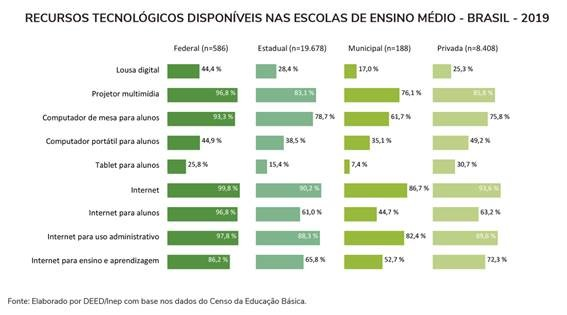
\includegraphics[scale=3.45]{./img/inep-grafico.png}
    \end{center}
    \legend{Fonte:\cite{INEP}}
  \end{figure}


  Com base nestas informações, é possível verificar boas oportunidades para as
  grandes e até pequenas empresas de software especializadas em criar sistemas e
  produtos focados para o ensino, uma aproximação com o setor público de educação
, reforça a importância de uma estratégia que estude as principais necessidades
  tecnológicas que este setor possui e com isso desenhar quais soluções,
  ferramentas e sistemas que seriam mais adequadas para suprir as carências por
  investimentos tecnológicos na educação pública no Brasil.

  \subsection{Empresas Privadas}

  Também importa ressaltar, que as instituições de ensino donas de escolas
  privadas possuem mais facilidade com relação ao poder de compra de softwares,
  isso é possível porque não necessitam de licitações fazendo com que a interação
  com as empresas desenvolvedoras de softwares seja mais dinâmica, abrindo
  caminho para o mercado tecnológico encontrar e promover soluções para o setor.

  \subsection{Instituições privadas sem fins lucrativos}

  O terceiro setor é composto por uma junção híbrida, entre empresas do setor
  privado e do setor público, cujo objetivo não é o lucro e sim atuar de forma
  voluntária e promover ações sociais destinadas ao interesse público. E neste
  grupo, algumas empresas precisam de recursos públicos ou doações para sustentar
  projetos e manter os trabalhos sociais.

  E porque a tecnologia é importante neste setor? Estas empresas não visam o
  lucro, mas precisam agir com transparência em relação a administração dos
  gastos, investimentos, divulgar ações, projetos referentes aos trabalhos que
  desenvolvem na sociedade. E para isso acontecer de forma clara é preciso tornar
  público todos os processos, que além de mostrar a verdade, possibilita aumentar
  a qualidade da prestação de serviços, buscar por novas tecnologias que tragam
  maior eficiência e representatividade ao setor.

  Quando estas instituições compram ou recebem através de doações um software, um
  sistema, um aplicativo para atender determinada atividade, elas podem ajudar a
  empresa que desenvolve o produto na divulgação da marca e da solução que aquele
  recurso oferece.  Desta maneira, seria possível influenciar outras empresas a
  adquirirem o software e expandir novos negócios tornando a atuação dentro deste
  setor cada vez mais forte, inclusive no Brasil hoje, a principal demanda da
  sociedade está voltada à prestação de serviços públicos para a área da educação
  e devido ao agravamento da pandemia, a saúde já necessitava de sistemas
  modernos, softwares e de serviços que permita fazer um acompanhamento dos casos
  com mais eficiência.

  \section{VIABILIDADE ECONÔMICA}

  No contexto deste projeto e da atual situação do Brasil, tendo em vista os
  dados apresentados no gráfico sobre recursos tecnológicos disponíveis nas
  escolas públicas do ensino médio e privado, analisar a viabilidade econômica do
  sistema que irá facilitar o empréstimo e a reserva de equipamentos e de
  positivos tecnológicos para professores e demais funcionários das escolas de
  ensino médio que disponibilizam estes recursos.

  Permite compreender, que a educação no Brasil ainda é deficitária no que tange
  aos investimentos e da aquisição de ferramentas tecnológicas, contudo este
  sistema seria uma solução viável economicamente, porque o processo para o
  desenvolvimento de software abrange conceitos e métodos focados na qualidade e
  na entrega de valor, ou seja, o propósito é que o sistema realize e cumpra os
  os objetivos para o qual ele foi desenvolvido e com o orçamento planejado
  possibilitando medir os custos incorridos ao longo do projeto e depois de
  pronto.

  Observando todos estes pontos, o produto é viável devido à utilidade prática
  dos recursos e pela oportunidade de negócios com o governo e com instituições
  de ensino privadas, pois ambas estão mais receptivas e perceberam que é
  importante direcionar esforços e investimentos em tecnologia para viabilizar a
  aprendizagem e potencializar o ensino.


  \subsection{Custos}

  Os custos podem ser estipulados como fixos: implantação, manutenção, suporte e
  outras despesas que podem incluir algumas variáveis como:

  \begin{itemize}
    \item Desenvolvimento (construção do software)
    \item Computadores (adquirir equipamentos para testes)
    \item Time interno (remunerar profissionais)
    \item Marketing (ações de  propaganda)
  \end{itemize}

  Seria importante avaliar os gastos com base em valores reais, considerando qual
  dos grupos, escolas do governo ou privadas, levantar os requisitos e estimar
  custos com base nos critérios de cada projeto por exemplo: o sistema é para
  facilitar a reserva de equipamentos digitais para os profissionais da escola
  utilizarem nas  aulas, palestras, apresentações e outros tipos de eventos. No
  entanto, o cliente quer adicionar uma nova funcionalidade ou fazer uma
  integração com outro sistema, então para cada implementação diferente irá
  variar o preço final do sistema.

  % ---
  % Conclusão
  % ---
  \section{CONCLUSÃO}

  Conclui-se que o software desenvolvido neste projeto vai ajudar e suprir a
  necessidade dos colégios em emprestar seus equipamentos e sendo de fácil
  manutenção por seguir o padrão ISO 9126 que tem como objetivo a qualidade do
  produto de software. Com boa documentação de testes manuais para evitar erros
  em produção deve ser estável e confiável.

  Seguindo uma interface simples e limpa o sistema pode ser utilizado por pessoas
  que precisam apenas saber o mínimo de informática não requisitado treinamento
  para a utilização, assim gerando uma economia com o corte de custo na
  implementação do sistema.

  Também foi feito uma análise sobre a viabilidade econômica e chegou à conclusão
  que os softwares ajudam no desenvolvimento do ensino, trazendo uma série de
  vantagens para tornar a educação mais disruptiva, saindo do convencional e
  simplificando a troca de aprendizagem.

  Além disso, as parcerias entre governos e instituições privadas de educação têm
  sido fundamental para acelerar os investimentos em tecnologias para o ensino e
  ao mesmo tempo incentivar que empresas de TI tenham oportunidades em aumentar
  seu portfólio de produtos e serviços focados neste mercado.

  Ainda é preciso mais estudos nesta área, no entanto muitas empresas de TI vem
  intensificando a oferta de seus produtos neste nicho porque embora tenhamos na
  realidade brasileira algumas desigualdades, onde a exclusão digital deve ser
  encarada como uma das paredes a serem quebradas.  Contudo, os avanços já são
  percebidos, de um lado o governo e as instituições privadas de ensino e
  empresas de tecnologia estão caminhando gradativamente sentido a transformação
  digital na educação de escolas públicas e privadas do país.
  % ----------------------------------------------------------
  % ELEMENTOS PÓS-TEXTUAIS
  % ----------------------------------------------------------
  \postextual

  % ----------------------------------------------------------
  % Referências bibliográficas
  % ----------------------------------------------------------
  \bibliography{abntex2-modelo-references.bib}


  % ----------------------------------------------------------
  % Glossário
  % ----------------------------------------------------------
  %
  % Consulte o manual da classe abntex2 para orientações sobre o glossário.
  %
  %\glossary



  % ----------------------------------------------------------
  % Anexos
  % ----------------------------------------------------------

  % ---
  % Inicia os anexos
  % ---

  %---------------------------------------------------------------------
  % INDICE REMISSIVO
  %---------------------------------------------------------------------

  \phantompart

  \printindex


  \end{document}
